%% Begin slides template file
\documentclass[11pt,t,usepdftitle=false,aspectratio=169]{beamer}
%% ------------------------------------------------------------------
%% - aspectratio=43: Set paper aspect ratio to 4:3.
%% - aspectratio=169: Set paper aspect ratio to 16:9.
%% ------------------------------------------------------------------

\usetheme[nototalframenumber,foot,logo]{uibk}

\title[]{Final presentation: Segfault Slayer}

\author[Schmölz Lukas, Schöpf Emanuel, Schweigl Dominik]{Schmölz Lukas, Schöpf Emanuel, Schweigl Dominik}

\headerimage{3}

\begin{document}

\section{Bookmark Title}
\subsection{Overview}


\begin{frame}
    \frametitle{Game Overview}

    \textbf{Game Idea}
    \begin{itemize}
        \item Metroidvania-style 2D side-scroller
        \item Player fights programming concepts and bugs
        \item Playful, Pixel-theme
    \end{itemize}

    \bigskip

    \textbf{World Design}
    \begin{itemize}
        \item First Area: Hardware with electric components roaming around
        \item Second Area: Abstract programming concepts escaped from the bosses lab
    \end{itemize}
\end{frame}


\begin{frame}{Used Tools}

    \textbf{Build Tools}
    \begin{itemize}
        \item SFML
        \item Tileson + Tiled
        \item Catch2
    \end{itemize}

    \bigskip

    \textbf{Asset Sources}
    \begin{itemize}
        \item Pixel art: Pixellab
        \item Audio: Pixabay (Sounds), itch.io (Music)
    \end{itemize}
\end{frame}


\begin{frame}{Boss Design}
    \begin{columns}[T]
        \begin{column}{0.4\textwidth}
            \vspace{2em}
            \small
            \textbf{Transistor}
            
            \begin{itemize}
                \item Roams the boss roam and shoots projectiles
                \item Shocks area around him when player too close
                \item Spawns additional minions in phase 2
            \end{itemize}

        \end{column}

        \begin{column}{0.6\textwidth}
        \vspace{-1em}
        \begin{figure}
            \centering
            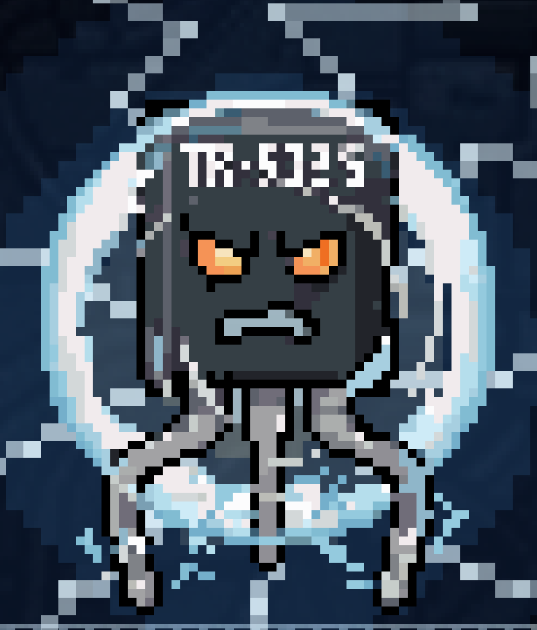
\includegraphics[width=0.6\linewidth]{_images/Transistor.png}
            \label{fig:segfault}
        \end{figure}

        \end{column}

    \end{columns}
\end{frame}


\begin{frame}{Boss Design}
    \begin{columns}[T]

        \begin{column}{0.6\textwidth}
            \vspace{-1em}
            \begin{figure}
                \centering
                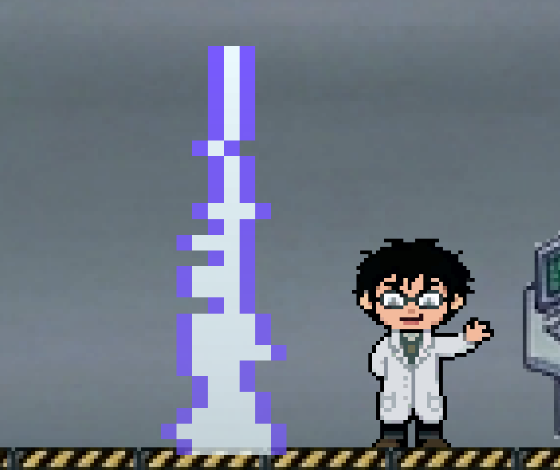
\includegraphics[width=0.8\linewidth]{_images/Segfault.png}
                \label{fig:segfault}
            \end{figure}
    
        \end{column}
    
        \begin{column}{0.4\textwidth}
            \vspace{2em}
            \small
            \textbf{Segfault}
            
            \begin{itemize}
                \item Spawns area attacks and environment blockers
                \item Summons minions in phase 2
                \item Glitches into 2 versions of himself in phase 3
            \end{itemize}

        \end{column}

    \end{columns}
\end{frame}


\begin{frame}[plain,c]
    \begin{center}
        \Huge{Demo \& Code Review}
    \end{center}
\end{frame}


\begin{frame}{Final Sprint}

    \begin{columns}[T]
        \begin{column}{0.4\textwidth}
            \vspace{2em}
            
            \begin{itemize}
                \item Last Music and Audio wiring
                \item Item \& enemy placement improvement
                \item Second Area rework
                \item Story snippets
                \item Refactoring
            \end{itemize}

        \end{column}

        \begin{column}{0.6\textwidth}
        \vspace{-1em}
        \begin{figure}
            \centering
            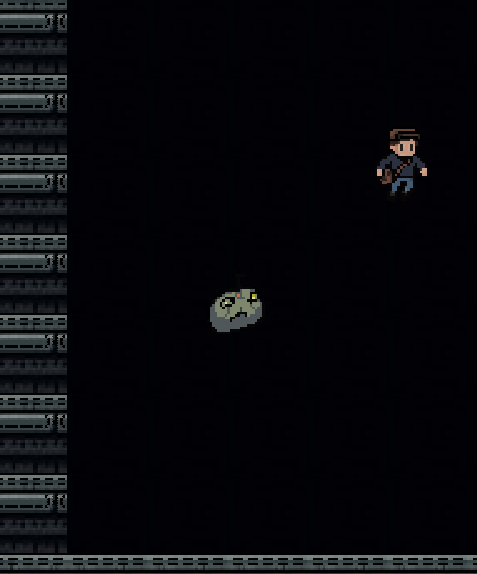
\includegraphics[width=0.6\linewidth]{_images/wall_jump.png}
            \label{fig:segfault}
        \end{figure}

        \end{column}

    \end{columns}

    \vspace{1em}

\end{frame}


\begin{frame}{Lessons Learned}
    \vspace{1em}

    
    \begin{itemize}
        \item Focus on creating a MVP early
        \item Creative Work just as important as gameplay mechanics
        \item Better Milestone / Issue Management
    \end{itemize}
\end{frame}

\end{document}
